\section{Results}
\label{sec:results}

Unless stated otherwise, model accuracy is measured on the $N = 2500$ held-out test scenarios. MAE, RMSE, and headline relative $L_2$ values are computed after reversing target normalization; max-err remains in normalized target units. The main model tables use the validated common-time evaluation; previously completed numerical-comparator studies and selected failure-case analyses are separately identified under the model-selection, dataset, and metric definitions stated in Sections~\ref{sec:methods}--\ref{sec:training}.

\subsection{Temporal alignment and numerical verification}
\label{subsec:res-dataset}

All three main datasets contain $10{,}000$ training, $1{,}000$ validation, and $2{,}500$ test scenarios. Each processed target has shape $50 \times 64 \times 64$, and all $40{,}500$ solver-specific trajectories pass the predefined quality checks. The scenario populations match across references: six source families, five bathymetry families, and resolved source strength in approximately $[0.075, 0.300]$ after the initial-elevation-to-depth cap.

Table~\ref{tab:solver-validation} summarizes the numerical evidence supporting the finite-horizon temporal-output procedure. It distinguishes current R6 checks from the earlier numerical program, whose artifacts are retained as historical provenance rather than relabeled as current validation.

\begin{table}[pos=htbp]
\centering
\caption{Numerical verification and inter-code comparison for the finite-horizon temporal-output procedure. This evidence assesses numerical consistency, not event-scale physical validity.}
\label{tab:solver-validation}
\small
\begin{tabular}{p{0.23\linewidth}p{0.55\linewidth}p{0.13\linewidth}}
    \toprule
    Evidence & Scope & Finding \\
    \midrule
    Current dataset and solver checks & $3$ datasets; all train/validation/test splits; $9$ representative solver cases & passed \\
    Shared inputs & $13{,}500$ scenarios; split identities, arrays, and horizon & matched across references \\
    Current R6 GeoClaw SWE comparison & $3$ fixed test cases; Hydrostatic and MUSCL-HR; $6$ comparisons & completed diagnostic \\
    Historical internal numerical checks & $86$ cases; $48$ analytical, numerical, and stability criteria & met criteria \\
    Historical GeoClaw/Clawpack comparisons & $3$ primary, $2$ verification, $7$ refinement, and $12$ exploratory cases & retained separately \\
    Historical integrated procedure checks & $90$ buffered common-time cases; $3$ repeatability checks & repeatable \\
    Historical H2 sensitivity checks & $363$ pairs; $726$ executions; $42$ fixed criteria & met criteria \\
    Dataset consistency checks & $3$ representative cases; $384 \rightarrow 128 \rightarrow 192 \rightarrow 64$ grid construction & passed \\
    \bottomrule
\end{tabular}
\end{table}

The current checks re-audited the three datasets across all train, validation, and test splits and reran nine representative solver cases. The fresh GeoClaw comparison then used the first R6 test case from each of three fixed terrain--source strata (continental/Gaussian, seamounts/fault, and trench/rough), selected before the GeoClaw outcomes were inspected. It verified the frozen input hashes, $192 \times 192$ state mapping, $128 \times 128$ central crop followed by $2 \times 2$ block averaging, all 50 requested times, and finite outputs. The historical analytical, refinement, and broader GeoClaw matrices remain separate evidence; they were not rerun under the current R6 contract.

\begin{table}[pos=htbp]
\centering
\caption{Current R6 inter-code comparison against GeoClaw over three fixed representative test cases. Both in-house references use the corrected $192 \times 192$ computation and reported $64 \times 64$ fields; GeoClaw receives the same frozen initial state and requested times. GeoClaw is an independent comparator, not physical truth.}
\label{tab:geoclaw-r6}
\small
\begin{tabular}{lcccc}
    \toprule
    In-house reference & Mean trajectory rel-$L_2$ & Range & Mean cosine similarity & Max gauge NRMSE \\
    \midrule
    Hydrostatic & $0.2599$ & $[0.2071,\,0.3326]$ & $0.9688$ & $0.2209$ \\
    MUSCL-HR & $0.1256$ & $[0.0659,\,0.1562]$ & $0.9914$ & $0.0865$ \\
    \bottomrule
\end{tabular}
\end{table}

Across these three current R6 cases, MUSCL-HR has the smaller descriptive discrepancy. The maximum initial-state mapping error is $8.9 \times 10^{-16}$ and the maximum requested-time mismatch is $5.7 \times 10^{-14}$, both far below the comparison tolerances. The comparison does not assign the residual to a single algorithmic choice: the implementations differ in boundary treatment, flux and source discretization, limiting, time integration, and CFL policy. It therefore neither establishes formal convergence nor pointwise equivalence.

The linear weakly dispersive reference also reproduces its discrete constant-depth phase-speed trend over eight Fourier modes. The maximum relative error is $2.45 \times 10 ^ {-4}$ for the non-dispersive branch and $1.91 \times 10 ^ {-8}$ for $\alpha_B = 1 / 3$, with no conjugate-gradient failures and at most $35$ iterations in the latter branch (Table~\ref{tab:app-bouss-dispersion}). This is a local numerical diagnostic rather than external or event-scale validation.

The central evaluation result is that reference discrepancy and surrogate error are on the same benchmark scale, but their ordering depends on the reference pair and architecture. As quantified in Section~\ref{subsec:res-solver-fidelity}, the Hydrostatic--MUSCL-HR gap is smaller than the selected direct Hydrostatic FNO and F-FNO RMSEs, whereas the cross-family gaps are comparable to or larger than the direct Boussinesq FNO RMSE. The architecture comparisons below therefore demonstrate the consequences of the reference-aware framework rather than defining its primary contribution.

\subsection{Direct same-reference accuracy}
\label{subsec:res-accuracy}

Table~\ref{tab:accuracy} contains the selected seed-$18$ results for all eleven direct model--reference configurations. Among the Hydrostatic configurations, ConvLSTM has the lowest global relative $L_2$ ($0.203$), followed by U-FNO ($0.224$) and F-FNO ($0.230$). The base FNO and its mode variants form a narrow $0.236$--$0.240$ group, while WNO, U-Net, and CNN are less accurate. F-FNO uses $0.411$M parameters, about $7.6\%$ as many as the $5.443$M-parameter FNO, so parameter count alone does not explain the observed ranking.

\begin{table}[pos=htbp]
\centering
\caption{Direct same-reference field accuracy on the held-out test split ($N = 2500$). Canonical sources are FNO and its mode variants \citep{li2021fno}, F-FNO \citep{tran2023ffno}, ConvLSTM \citep{shi2015convlstm}, U-FNO \citep{wen2022ufno}, WNO \citep{tripura2023wno}, U-Net \citep{ronneberger2015unet}, and the general CNN precedent \citep{lecun1998gradient}; the reported implementations are defined in Section~\ref{sec:models}. Params are millions. MAE, RMSE, and relative $L_2$ are in the denormalized benchmark space; max-err is the global normalized-unit maximum.}
\label{tab:accuracy}
\small
\begin{tabular}{llccccc}
    \toprule
    Model & Reference & Params & MAE & RMSE & rel-$L_2$ & max-err \\
    \midrule
    ConvLSTM    & Hydrostatic & $0.359$  & $0.00094$ & $0.00179$ & $\mathbf{0.203}$ & $13.5$ \\
    U-FNO       & Hydrostatic & $6.938$  & $0.00111$ & $0.00197$ & $0.224$ & $10.7$ \\
    F-FNO       & Hydrostatic & $0.411$  & $0.00118$ & $0.00203$ & $0.230$ & $9.7$ \\
    FNO-modes8  & Hydrostatic & $1.793$  & $0.00120$ & $0.00208$ & $0.236$ & $9.7$ \\
    FNO-modes20 & Hydrostatic & $11.083$ & $0.00126$ & $0.00211$ & $0.240$ & $10.7$ \\
    FNO         & Hydrostatic & $5.443$  & $0.00126$ & $0.00212$ & $0.240$ & $11.1$ \\
    WNO         & Hydrostatic & $2.016$  & $0.00196$ & $0.00321$ & $0.364$ & $12.6$ \\
    U-Net       & Hydrostatic & $0.104$  & $0.00249$ & $0.00407$ & $0.462$ & $10.8$ \\
    CNN         & Hydrostatic & $0.045$  & $0.00316$ & $0.00512$ & $0.581$ & $12.4$ \\
    \midrule
    FNO         & MUSCL-HR    & $5.443$  & $0.00160$ & $0.00257$ & $0.268$ & $13.1$ \\
    FNO         & Boussinesq  & $5.443$  & $0.00196$ & $0.00302$ & $0.285$ & $17.1$ \\
    \bottomrule
\end{tabular}
\end{table}

The Boussinesq FNO has a larger relative $L_2$ than the Hydrostatic FNO and a similar denormalized RMSE to the raw cross-family gaps. This is why the reference-specific ranking must not be reduced to one number: target scale and waveform structure differ across equation families.

\paragraph{Paired scenario uncertainty.}
The paired scenario bootstrap gives mean per-scenario relative $L_2$ values of $0.250$ ($95\%$ interval $[0.246, 0.255]$) for F-FNO, $0.208$ ($[0.203, 0.212]$) for ConvLSTM, and $0.270$ ($[0.265, 0.275]$) for FNO. Relative to FNO, the paired mean differences are $-0.020$ ($[-0.022, -0.017]$) for F-FNO and $-0.062$ ($[-0.066, -0.059]$) for ConvLSTM. Their per-scenario errors are lower than FNO on $63.9\%$ and $79.4\%$ of the test scenarios, respectively. These intervals describe variation over the fixed test scenarios for the selected checkpoints; they are not training-seed significance claims.

For the seed-$18$ global metric in Table~\ref{tab:accuracy}, ConvLSTM improves Hydrostatic relative $L_2$ by approximately $15\%$ relative to FNO, while F-FNO uses about $7.6\%$ as many parameters as FNO. ConvLSTM also has the lowest final-frame error among the three models shown in Table~\ref{tab:perframe}. Figure~\ref{fig:rollout} illustrates one direct Hydrostatic FNO rollout at the first, middle, and final requested times. These are fixed-checkpoint results rather than broad population-level architecture claims.

\begin{figure}[pos=htbp]
\centering

\includegraphics[width=0.72\linewidth]{figures/hydrostatic_rollout.pdf}
\caption{Direct FNO prediction for common-time Hydrostatic test scenario \texttt{scenario\_001302}, a continental/Okada-like pair selected near the test-split median error. Reference, prediction, and absolute error are shown at $t = 8.4$, $210.0$, and $420.0$ in elapsed benchmark-time units. All $\eta$ panels are denormalized benchmark-scale fields.}
\label{fig:rollout}
\end{figure}

\paragraph{Per-frame behavior.}
Table~\ref{tab:perframe} reports denormalized benchmark-scale relative $L_2$ at the first, middle, and final requested times. Errors generally grow over the horizon, with ConvLSTM showing the flattest selected curve and the Boussinesq FNO also increasing substantially by the final frame.

\begin{table}[pos=htbp]
\centering
\caption{Per-frame denormalized benchmark-scale relative $L_2$ on the $N = 2500$ test split.}
\label{tab:perframe}
\begin{tabular}{llccc}
    \toprule
    Model & Reference & frame $1$ & frame $25$ & frame $50$ \\
    \midrule
    F-FNO    & Hydrostatic & $0.205$ & $0.255$ & $0.327$ \\
    ConvLSTM & Hydrostatic & $0.197$ & $0.214$ & $0.217$ \\
    FNO      & Hydrostatic & $0.214$ & $0.269$ & $0.339$ \\
    FNO      & MUSCL-HR    & $0.216$ & $0.310$ & $0.414$ \\
    FNO      & Boussinesq  & $0.218$ & $0.320$ & $0.404$ \\
    \bottomrule
\end{tabular}
\end{table}

\paragraph{Physics diagnostics.}
Table~\ref{tab:physics-diag} compares the Hydrostatic integral and spectral diagnostics. ConvLSTM has the lowest integral, low-frequency, and mid-frequency errors among the three diagnostic models. F-FNO improves the low-frequency error relative to FNO but has larger mid- and high-frequency errors. These quantities diagnose where the error lies; they do not imply conservation enforcement.

\begin{table}[pos=htbp]
\centering
\caption{Hydrostatic denormalized benchmark-scale diagnostics on the full test split. Integral columns are relative $L_2$ of spatial-mean time series; spectral columns are bandwise field relative $L_2$.}
\label{tab:physics-diag}
\begin{tabular}{lccccc}
    \toprule
    Model & $\eta$ integral & mass proxy & low & mid & high \\
    \midrule
    FNO      & $0.203$ & $1.29 \times 10 ^ {-4}$ & $0.231$ & $0.397$ & $0.372$ \\
    F-FNO    & $0.195$ & $1.24 \times 10 ^ {-4}$ & $0.220$ & $0.479$ & $0.426$ \\
    ConvLSTM & $0.194$ & $1.24 \times 10 ^ {-4}$ & $0.199$ & $0.357$ & $0.375$ \\
    \bottomrule
\end{tabular}
\end{table}

\subsection{Runtime comparison}
\label{subsec:res-speed}

Table~\ref{tab:speed} reports matched reference and batch-one inference timings. The float64 CPU reference rollouts take $19.923$~s for Hydrostatic, $30.318$~s for MUSCL-HR, and $16.457$~s for Boussinesq per sample. Direct GPU inference ranges from $0.138$~ms for CNN to $22.190$~ms for ConvLSTM. Comparing only the forward calculations, the measured ratios range from $898 \times$ to $144{,}170 \times$ across the reported models.

\begin{table}[pos=htbp]
\centering
\caption{Batch-one model inference time on the laptop GPU versus the matched float64 CPU common-time reference rollout. Model timing uses five warm-up and twenty measured passes with TF32 disabled; each solver mean uses eight scenarios, one warm-up, and three measured repeats. Loading, input preparation, and solver setup are excluded from the comparison.}
\label{tab:speed}
\small
\begin{tabular}{lccrr}
    \toprule
    Model & Reference & model time (ms) & reference time (s) & ratio \\
    \midrule
    FNO         & Hydrostatic & $1.162$ & $19.923$ & $17{,}148  \times$ \\
    F-FNO       & Hydrostatic & $1.364$ & $19.923$ & $14{,}604  \times$ \\
    CNN         & Hydrostatic & $0.138$ & $19.923$ & $144{,}170 \times$ \\
    U-Net       & Hydrostatic & $0.186$ & $19.923$ & $106{,}895 \times$ \\
    ConvLSTM    & Hydrostatic & $22.190$ & $19.923$ & $898      \times$ \\
    U-FNO       & Hydrostatic & $3.710$ & $19.923$ & $5{,}370   \times$ \\
    WNO         & Hydrostatic & $1.719$ & $19.923$ & $11{,}590  \times$ \\
    FNO-modes8  & Hydrostatic & $1.172$ & $19.923$ & $16{,}996  \times$ \\
    FNO-modes20 & Hydrostatic & $2.072$ & $19.923$ & $9{,}615   \times$ \\
    FNO         & MUSCL-HR    & $1.189$ & $30.318$ & $25{,}491  \times$ \\
    FNO         & Boussinesq  & $1.159$ & $16.457$ & $14{,}198  \times$ \\
    \bottomrule
\end{tabular}
\end{table}

These ratios reflect the particular CPU and laptop-GPU implementations used in this study. They should not be interpreted as speedups over operational, compiled, GPU, or adaptive-mesh solvers.

\subsection{Distribution shift and sample scaling}
\label{subsec:res-ood}

Table~\ref{tab:ood} groups the Hydrostatic FNO by source family using means of per-scenario denormalized benchmark-scale relative $L_2$. Dipole sources are the hardest group ($0.330$), while the other families lie between $0.236$ and $0.293$. The bathymetry grouping identifies continental fields as the hardest family ($0.317$). Because every family appears in training, these are subgroup diagnostics, not unseen-family tests.

\begin{table}[pos=htbp]
\centering
\caption{Hydrostatic FNO source-family subgroups. Metrics are means of per-scenario denormalized benchmark-scale values.}
\label{tab:ood}
\begin{tabular}{lcc}
    \toprule
    Source family & rel-$L_2$ & $n$ \\
    \midrule
    multi-gauss & $0.236$ & $410$ \\
    gaussian    & $0.241$ & $466$ \\
    fault       & $0.252$ & $379$ \\
    rough       & $0.271$ & $419$ \\
    okada-like  & $0.293$ & $423$ \\
    dipole      & $\mathbf{0.330}$ & $403$ \\
    \bottomrule
\end{tabular}
\end{table}

The strict holdouts in Table~\ref{tab:strict-holdout} are more demanding for some families. The held-out/ID relative-$L_2$ ratios are $1.02$ for trench, $2.15$ for continental bathymetry, $1.33$ for rough sources, and $1.12$ for Okada-like sources. The full-distribution model is better on every excluded family, indicating that removing the family costs more than any benefit from specializing the normalization and training distribution. This remains a single-seed comparison and does not separate representation limits from reduced training-set diversity.

\begin{table}[pos=htbp]
\centering
    \caption{Strict Hydrostatic FNO held-out-family tests. Values are denormalized benchmark-scale relative $L_2$ after applying the normalization statistics associated with each model.}
\label{tab:strict-holdout}
\begin{tabular}{lccccc}
    \toprule
    Held-out family & $n_{\mathrm{ID}}$ & $n_{\mathrm{HO}}$ & ID & held-out & full model / ratio \\
    \midrule
    \texttt{trench} bathymetry      & $2016$ & $484$ & $0.251$ & $0.258$ & $0.229$ / $1.02$ \\
    \texttt{continental} bathymetry & $2002$ & $498$ & $0.235$ & $0.506$ & $0.282$ / $2.15$ \\
    \texttt{rough} source           & $2081$ & $419$ & $0.241$ & $0.319$ & $0.265$ / $1.33$ \\
    \texttt{okada-like} source      & $2077$ & $423$ & $0.241$ & $0.270$ & $0.246$ / $1.12$ \\
    \bottomrule
\end{tabular}
\end{table}

The six seed-$18$ sample-scaling experiments are monotone: relative $L_2$ falls from $0.544$ with $100$ training scenarios to $0.259$ with $5{,}000$, while the $10{,}000$-scenario direct FNO reaches $0.240$. Full values and curves are given in Appendix~\ref{app:sample-scaling}; this is a diagnostic learning curve, not a fitted scaling law.

\subsection{Resolution transfer}
\label{subsec:res-crossres}

Table~\ref{tab:crossres} reports the proxy Hydrostatic experiment, which applies the same FNO trained at $64 \times 64$ after resizing the processed test fields. Error rises in both directions, to $0.396$ at $32 \times 32$ and $0.364$ at $128 \times 128$.

\begin{table}[pos=htbp]
\centering
\caption{Proxy Hydrostatic FNO resolution transfer ($ N = 2500$). The $64 \times 64$ row is the ordinary test set.}
\label{tab:crossres}
\begin{tabular}{lccc}
    \toprule
    Evaluation grid & MAE & RMSE & rel-$L_2$ \\
    \midrule
    $32  \times 32$  proxy  & $0.00237$ & $0.00349$ & $0.396$ \\
    $64  \times 64$  native & $0.00126$ & $0.00212$ & $0.240$ \\
    $128 \times 128$ proxy  & $0.00213$ & $0.00320$ & $0.364$ \\
    \bottomrule
\end{tabular}
\end{table}

The stronger native experiment in Table~\ref{tab:crossres-native-transfer} uses paired MUSCL-HR simulations and three separately trained models. The diagonal errors are $0.353$, $0.387$, and $0.412$ for $32$, $64$, and $128$ grids. Off-diagonal transfer is consistently worse than the corresponding diagonal, with the largest degradation from $32$-grid training to the $128$-grid test.

\begin{table}[pos=htbp]
\centering
\caption{Native MUSCL-HR FNO transfer matrix. Rows are training grids and columns are native test grids; each cell is denormalized benchmark-scale relative $L_2$ on $150$ matched scenarios.}
\label{tab:crossres-native-transfer}
\begin{tabular}{lccc}
    \toprule
    Train grid & Test $32$ & Test $64$ & Test $128$ \\
    \midrule
    $32$  & $\mathbf{0.353}$ & $0.670$ & $0.808$ \\
    $64$  & $0.473$ & $\mathbf{0.387}$ & $0.530$ \\
    $128$ & $0.591$ & $0.433$ & $\mathbf{0.412}$ \\
    \bottomrule
\end{tabular}
\end{table}

Each native model sees only $700$ training scenarios, so the matrix should not be compared directly with the main $10{,}000$-scenario Hydrostatic model as though resolution were the only variable.

\subsection{Synthetic-forcing transfer to real bathymetry}
\label{subsec:res-real}

Table~\ref{tab:real-bath} summarizes the main morphology suite of ten GEBCO-derived fully wet crops rescaled into the training depth range and paired with synthetic sources, while Figure~\ref{fig:real-bath} illustrates one offshore crop at the final requested time. Direct F-FNO transfers better than direct FNO, with denormalized benchmark-scale relative $L_2$ $0.293$ versus $0.358$. The seeded window results are lower but are not like-for-like direct forecasts.

\begin{table}[pos=htbp]
\centering
\caption{Real-bathymetry morphology suite under synthetic forcing. Window models receive the first true target frame and are scored on the remaining $49$ frames.}
\label{tab:real-bath}
\begin{tabular}{lccc}
    \toprule
    Model & Samples & normalized rel-$L_2$ & denormalized rel-$L_2$ \\
    \midrule
    Direct FNO       & $10$ & $0.364$ & $0.358$ \\
    Direct F-FNO     & $10$ & $0.299$ & $0.293$ \\
    Window-FNO-5     & $10$ & $0.067$ & $0.066$ \\
    Window-F-FNO-5   & $10$ & $0.064$ & $0.063$ \\
    \bottomrule
\end{tabular}
\end{table}

\begin{figure}[pos=htbp]
\centering

\includegraphics[width=0.72\linewidth]{figures/real_bathymetry_offshore.pdf}
\caption{Synthetic-forcing morphology transfer on one illustrative fully wet offshore crop derived from the GEBCO\_2026 Grid \citep{gebco2026}. At the final requested time, the figure compares the reference field with direct-FNO and first-frame-seeded Window-FNO-5 errors. Their full-trajectory denormalized benchmark-scale relative $L_2$ values are $0.212$ and $0.035$. This is not real-event validation.}
\label{fig:real-bath}
\end{figure}

The fully wet coastline ablation remains usable, but the coastline stress case with positive topography gives relative $L_2$ near one for all four models. This isolates a clear scope boundary: transfer to offshore morphology does not imply shoreline or wet--dry skill.

\subsection{Common-time solver gaps and cross-reference ratios}
\label{subsec:res-solver-fidelity}

Table~\ref{tab:solvergap} reports the common-time solver discrepancies. The Hydrostatic--MUSCL-HR gap is the smallest pairwise discrepancy: its global field RMSE is $0.00171$, compared with $0.00305$ and $0.00374$ for the two shallow-water--Boussinesq pairs. The relative $L_2$ is directional because it divides by the second reference's norm.

\begin{table}[pos=htbp]
\centering
\caption{Common-time solver gaps on all $2500$ shared test scenarios. Scenario metrics are means with the second solver as the relative-$L_2$ reference.}
\label{tab:solvergap}
\begin{tabular}{llccc}
    \toprule
    Solver $A$ & Solver $B$ & global RMSE & mean scenario RMSE & mean rel-$L_2$ \\
    \midrule
    Hydrostatic & MUSCL-HR   & $0.00171$ & $0.00149$ & $0.188$ \\
    Hydrostatic & Boussinesq & $0.00374$ & $0.00322$ & $0.357$ \\
    MUSCL-HR    & Boussinesq & $0.00305$ & $0.00254$ & $0.279$ \\
    \bottomrule
\end{tabular}
\end{table}

Figure~\ref{fig:solver-gap-scale} places the same-reference errors of the Hydrostatic FNO, Hydrostatic F-FNO, and Boussinesq FNO alongside the raw solver gaps on one denormalized RMSE scale. The Hydrostatic--MUSCL-HR gap is $0.81$ and $0.84$ times the Hydrostatic FNO and F-FNO RMSEs, respectively. The Hydrostatic--Boussinesq and MUSCL-HR--Boussinesq gaps are $1.24$ and $1.01$ times the Boussinesq FNO RMSE.

\begin{figure}[pos=htbp]
\centering
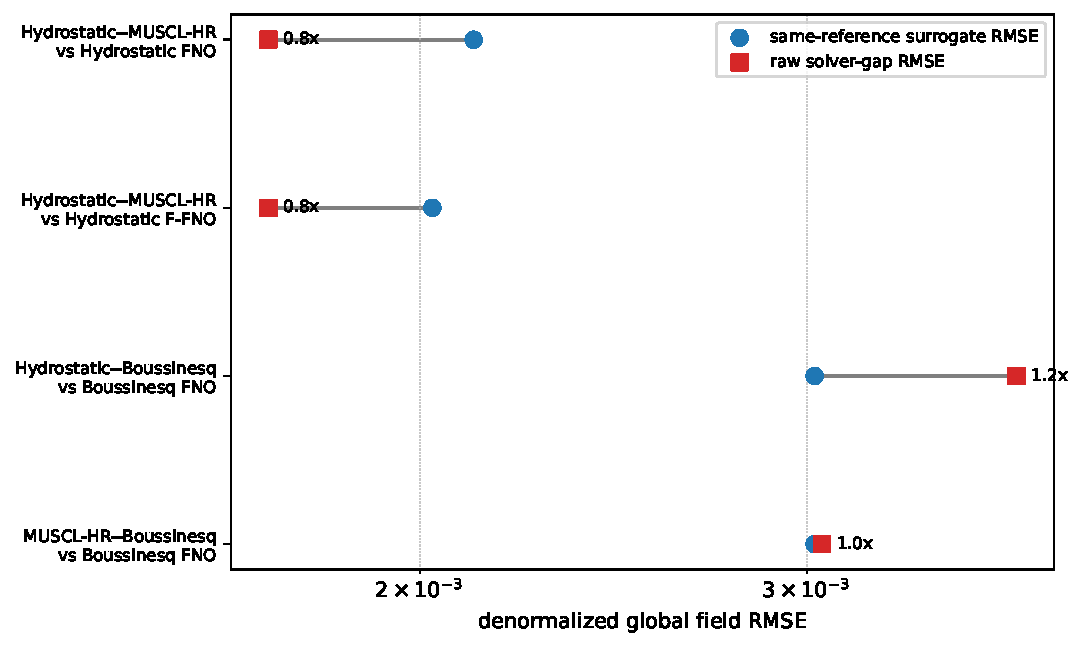
\includegraphics[width=0.88\linewidth]{figures/solver_gap_vs_surrogate_error.pdf}
\caption{Raw common-time solver gaps compared with the same-reference errors of the Hydrostatic FNO, Hydrostatic F-FNO, and Boussinesq FNO in the same denormalized global-RMSE units. Lines connect each surrogate error to its paired solver gap; annotations give the gap-to-surrogate ratio.}
\label{fig:solver-gap-scale}
\end{figure}

Table~\ref{tab:superiority} reports all six directions for the selected seed-$18$ checkpoints. Every ratio exceeds one, ranging from $1.10$ to $1.72$, so none of the tested emulators bridges its raw solver gap in this global-RMSE metric.

\begin{table}[pos=htbp]
\centering
\caption{Seed-$18$ cross-reference discrepancy ratio $\rho$ with $95\%$ paired scenario-bootstrap intervals. Values below one would mean closer to the second numerical reference in global RMSE, not physical superiority.}
\label{tab:superiority}
\small
\begin{tabular}{llc}
    \toprule
    Trained on & Compared with & $\rho$ [$95\%$ CI] \\
    \midrule
    Hydrostatic & MUSCL-HR    & $1.723$ $[1.701, 1.747]$ \\
    MUSCL-HR    & Hydrostatic & $1.544$ $[1.511, 1.580]$ \\
    Hydrostatic & Boussinesq  & $1.201$ $[1.192, 1.209]$ \\
    MUSCL-HR    & Boussinesq  & $1.347$ $[1.332, 1.361]$ \\
    Boussinesq  & Hydrostatic & $1.097$ $[1.079, 1.115]$ \\
    Boussinesq  & MUSCL-HR    & $1.297$ $[1.275, 1.319]$ \\
    \bottomrule
\end{tabular}
\end{table}

The cross-family effects are smaller than the shallow-water-direction ratios but remain above one in the present comparison. Thus the strongest statement supported by these results is that all six tested directions retain a larger emulator-to-reference discrepancy than the corresponding raw solver gap; this is a benchmark-relative result, not evidence that any reference is physically more accurate.

Figure~\ref{fig:cross-reference-forest} shows the seed-$18$ ratios with their paired scenario-bootstrap intervals. The reference line at $\rho = 1$ is the raw solver-gap scale; Table~\ref{tab:superiority} separately reports training-seed variation.

\begin{figure}[pos=htbp]
\centering
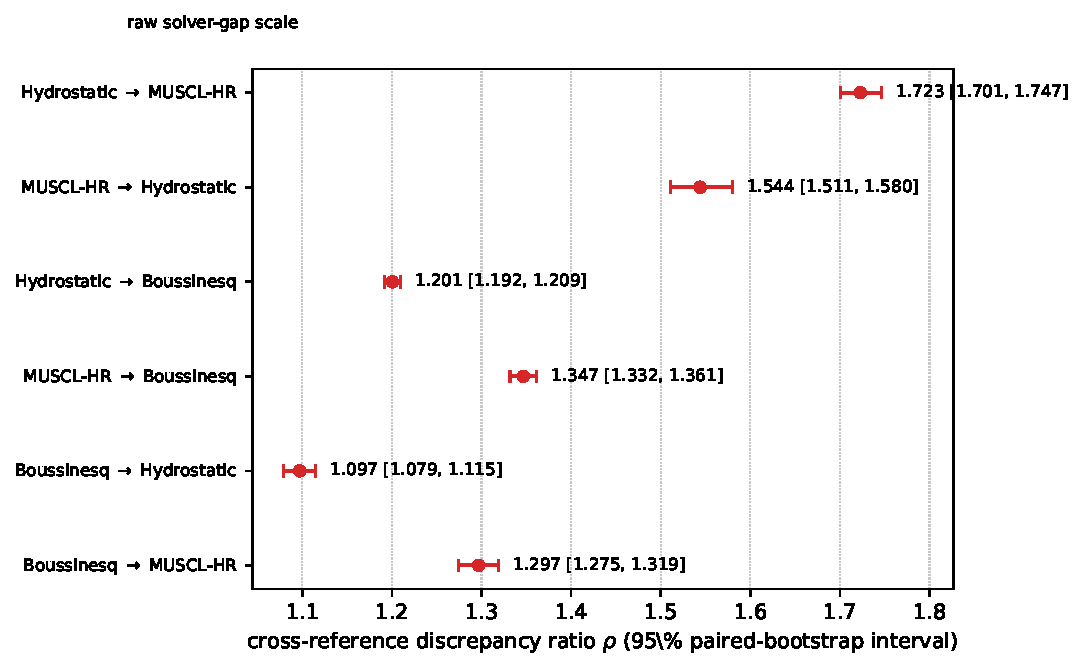
\includegraphics[width=0.88\linewidth]{figures/cross_reference_ratio_forest.pdf}
\caption{Seed-$18$ cross-reference discrepancy ratios with $95\%$ paired scenario-bootstrap intervals. The dashed line denotes equality with the corresponding raw solver gap, not equality with physical truth.}
\label{fig:cross-reference-forest}
\end{figure}

\subsection{Gauge, arrival, and peak diagnostics}
\label{subsec:res-wave}

Table~\ref{tab:wave-metrics} summarizes nine virtual gauges per scenario. Waveform NRMSE increases from Hydrostatic to MUSCL-HR to Boussinesq, while median arrival and time-to-peak errors are $25.2$ and $4.2$ benchmark-time units for all three targets. The compared arrival counts are $6{,}545$, $6{,}927$, and $7{,}050$ after excluding gauges already active at the first requested time; no missing predicted arrivals were recorded. The eligibility difference is therefore a property of the target waveforms and threshold policy, not a shortage of virtual gauges.

\begin{table}[pos=htbp]
\centering
\caption{FNO virtual-gauge diagnostics. Arrival errors use only eligible target gauges; time values are normalized benchmark-time units.}
\label{tab:wave-metrics}
\small
\setlength{\tabcolsep}{3pt}
\begin{tabular}{lccccc}
    \toprule
    Reference & \shortstack{waveform NRMSE\\median / p95} & \shortstack{compared\\arrivals} & \shortstack{arrival abs.\\median} & \shortstack{peak abs.\\median} & \shortstack{time-to-peak\\median} \\
    \midrule
    Hydrostatic & $0.106$ / $0.309$ & $6545$ & $25.2$ & $0.00204$ & $4.2$ \\
    MUSCL-HR    & $0.119$ / $0.329$ & $6927$ & $25.2$ & $0.00237$ & $4.2$ \\
    Boussinesq  & $0.134$ / $0.346$ & $7050$ & $25.2$ & $0.00250$ & $4.2$ \\
    \bottomrule
\end{tabular}
\end{table}

The pixelwise arrival maps give mean per-scenario eligible-pixel absolute differences of $1.16$, $1.43$, and $1.79$ requested-time indices for Hydrostatic, MUSCL-HR, and Boussinesq, respectively. Their mean valid-arrival fractions are $0.84$, $0.91$, and $0.92$. These values average scenario-level errors rather than pooling all eligible cells, so they should be interpreted together with the aggregation rule and eligibility context.

\paragraph{Conditional windowed forecasts.}
First-target-frame-seeded Window-FNO-5 and Window-F-FNO-5 provide long-horizon drift diagnostics, but they solve an easier conditional task than the direct $50$-frame forecast. Their full metrics and speed--accuracy trade-off are therefore retained in Table~\ref{tab:app-window} rather than included in the primary model comparison.

\subsection{Ensemble uncertainty and seed stability}
\label{subsec:res-uncertainty}

Table~\ref{tab:uncertainty} summarizes the seven-member ensemble reliability. The raw ensemble is under-dispersed: on the ordinary test split, coverage is $0.368$, $0.591$, $0.682$, and $0.743$ for nominal $50\%$, $80\%$, $90\%$, and $95\%$ intervals. The error--uncertainty correlation is $0.496$, indicating useful but only moderate spatial ranking.

A validation-only variance multiplier $\gamma = 4.995$ (standard-deviation scale $2.235$) raises test $90\%$ coverage from $0.682$ to $0.910$. It also improves the multi-Gaussian subgroup from $0.613$ to $0.877$ and trench from $0.697$ to $0.918$, while the high-strength tail remains under-covered at $0.796$.

\begin{table}[pos=htbp]
\centering
\caption{Seven-member FNO ensemble reliability. Coverage is marginal over correlated pixels and frames.}
\label{tab:uncertainty}
\begin{tabular}{lcccc}
    \toprule
    Suite & $n$ & err--unc.\ corr. & raw cov$_{90}$ & scaled cov$_{90}$ \\
    \midrule
    Validation & $1000$ & $0.492$ & $0.688$ & $0.914$ \\
    Test & $2500$ & $0.496$ & $0.682$ & $0.910$ \\
    \texttt{multi-gauss} subgroup & $410$ & $0.463$ & $0.613$ & $0.877$ \\
    \texttt{trench} subgroup & $484$ & $0.436$ & $0.697$ & $0.918$ \\
    high-strength subgroup & $177$ & $0.550$ & $0.512$ & $0.796$ \\
    \bottomrule
\end{tabular}
\end{table}

Across the seven individual seeds, the mean per-scenario relative $L_2$ ranges from $0.257$ to $0.273$, with member mean $0.265$ and standard deviation $0.0055$. This seven-member set supports the Hydrostatic FNO uncertainty analysis; it is not a replicated architecture comparison.

Variance inflation improves interval scale but does not make the ensemble uniformly calibrated. The corrected test coverage is close to nominal at $90\%$, while the high-strength subgroup remains about ten percentage points below nominal. Together with the moderate error--uncertainty correlation, this supports using ensemble spread as a relative diagnostic within the benchmark rather than as a calibrated hazard probability.
